% Options for packages loaded elsewhere
\PassOptionsToPackage{unicode}{hyperref}
\PassOptionsToPackage{hyphens}{url}
\PassOptionsToPackage{dvipsnames,svgnames,x11names}{xcolor}
%
\documentclass[
  letterpaper,
]{article}

\usepackage{amsmath,amssymb}
\usepackage{lmodern}
\usepackage{iftex}
\ifPDFTeX
  \usepackage[T1]{fontenc}
  \usepackage[utf8]{inputenc}
  \usepackage{textcomp} % provide euro and other symbols
\else % if luatex or xetex
  \usepackage{unicode-math}
  \defaultfontfeatures{Scale=MatchLowercase}
  \defaultfontfeatures[\rmfamily]{Ligatures=TeX,Scale=1}
  \setmainfont[]{Latin Modern Roman}
  \setmathfont[]{Latin Modern Math}
\fi
% Use upquote if available, for straight quotes in verbatim environments
\IfFileExists{upquote.sty}{\usepackage{upquote}}{}
\IfFileExists{microtype.sty}{% use microtype if available
  \usepackage[]{microtype}
  \UseMicrotypeSet[protrusion]{basicmath} % disable protrusion for tt fonts
}{}
\makeatletter
\@ifundefined{KOMAClassName}{% if non-KOMA class
  \IfFileExists{parskip.sty}{%
    \usepackage{parskip}
  }{% else
    \setlength{\parindent}{0pt}
    \setlength{\parskip}{6pt plus 2pt minus 1pt}}
}{% if KOMA class
  \KOMAoptions{parskip=half}}
\makeatother
\usepackage{xcolor}
\setlength{\emergencystretch}{3em} % prevent overfull lines
\setcounter{secnumdepth}{2}
% Make \paragraph and \subparagraph free-standing
\ifx\paragraph\undefined\else
  \let\oldparagraph\paragraph
  \renewcommand{\paragraph}[1]{\oldparagraph{#1}\mbox{}}
\fi
\ifx\subparagraph\undefined\else
  \let\oldsubparagraph\subparagraph
  \renewcommand{\subparagraph}[1]{\oldsubparagraph{#1}\mbox{}}
\fi


\providecommand{\tightlist}{%
  \setlength{\itemsep}{0pt}\setlength{\parskip}{0pt}}\usepackage{longtable,booktabs,array}
\usepackage{calc} % for calculating minipage widths
% Correct order of tables after \paragraph or \subparagraph
\usepackage{etoolbox}
\makeatletter
\patchcmd\longtable{\par}{\if@noskipsec\mbox{}\fi\par}{}{}
\makeatother
% Allow footnotes in longtable head/foot
\IfFileExists{footnotehyper.sty}{\usepackage{footnotehyper}}{\usepackage{footnote}}
\makesavenoteenv{longtable}
\usepackage{graphicx}
\makeatletter
\def\maxwidth{\ifdim\Gin@nat@width>\linewidth\linewidth\else\Gin@nat@width\fi}
\def\maxheight{\ifdim\Gin@nat@height>\textheight\textheight\else\Gin@nat@height\fi}
\makeatother
% Scale images if necessary, so that they will not overflow the page
% margins by default, and it is still possible to overwrite the defaults
% using explicit options in \includegraphics[width, height, ...]{}
\setkeys{Gin}{width=\maxwidth,height=\maxheight,keepaspectratio}
% Set default figure placement to htbp
\makeatletter
\def\fps@figure{htbp}
\makeatother
\newlength{\cslhangindent}
\setlength{\cslhangindent}{1.5em}
\newlength{\csllabelwidth}
\setlength{\csllabelwidth}{3em}
\newlength{\cslentryspacingunit} % times entry-spacing
\setlength{\cslentryspacingunit}{\parskip}
\newenvironment{CSLReferences}[2] % #1 hanging-ident, #2 entry spacing
 {% don't indent paragraphs
  \setlength{\parindent}{0pt}
  % turn on hanging indent if param 1 is 1
  \ifodd #1
  \let\oldpar\par
  \def\par{\hangindent=\cslhangindent\oldpar}
  \fi
  % set entry spacing
  \setlength{\parskip}{#2\cslentryspacingunit}
 }%
 {}
\usepackage{calc}
\newcommand{\CSLBlock}[1]{#1\hfill\break}
\newcommand{\CSLLeftMargin}[1]{\parbox[t]{\csllabelwidth}{#1}}
\newcommand{\CSLRightInline}[1]{\parbox[t]{\linewidth - \csllabelwidth}{#1}\break}
\newcommand{\CSLIndent}[1]{\hspace{\cslhangindent}#1}

\usepackage{arxiv}
\usepackage{orcidlink}
\usepackage{amsmath}
\usepackage[T1]{fontenc}
\makeatletter
\makeatother
\makeatletter
\makeatother
\makeatletter
\@ifpackageloaded{caption}{}{\usepackage{caption}}
\AtBeginDocument{%
\ifdefined\contentsname
  \renewcommand*\contentsname{Table of contents}
\else
  \newcommand\contentsname{Table of contents}
\fi
\ifdefined\listfigurename
  \renewcommand*\listfigurename{List of Figures}
\else
  \newcommand\listfigurename{List of Figures}
\fi
\ifdefined\listtablename
  \renewcommand*\listtablename{List of Tables}
\else
  \newcommand\listtablename{List of Tables}
\fi
\ifdefined\figurename
  \renewcommand*\figurename{Figure}
\else
  \newcommand\figurename{Figure}
\fi
\ifdefined\tablename
  \renewcommand*\tablename{Table}
\else
  \newcommand\tablename{Table}
\fi
}
\@ifpackageloaded{float}{}{\usepackage{float}}
\floatstyle{ruled}
\@ifundefined{c@chapter}{\newfloat{codelisting}{h}{lop}}{\newfloat{codelisting}{h}{lop}[chapter]}
\floatname{codelisting}{Listing}
\newcommand*\listoflistings{\listof{codelisting}{List of Listings}}
\makeatother
\makeatletter
\@ifpackageloaded{caption}{}{\usepackage{caption}}
\@ifpackageloaded{subcaption}{}{\usepackage{subcaption}}
\makeatother
\makeatletter
\@ifpackageloaded{tcolorbox}{}{\usepackage[many]{tcolorbox}}
\makeatother
\makeatletter
\@ifundefined{shadecolor}{\definecolor{shadecolor}{rgb}{.97, .97, .97}}
\makeatother
\makeatletter
\makeatother
\ifLuaTeX
  \usepackage{selnolig}  % disable illegal ligatures
\fi
\IfFileExists{bookmark.sty}{\usepackage{bookmark}}{\usepackage{hyperref}}
\IfFileExists{xurl.sty}{\usepackage{xurl}}{} % add URL line breaks if available
\urlstyle{same} % disable monospaced font for URLs
\hypersetup{
  pdftitle={A Simple Simulation of Ridehail Systems},
  pdfauthor={Tom Slee},
  colorlinks=true,
  linkcolor={blue},
  filecolor={Maroon},
  citecolor={Blue},
  urlcolor={Blue},
  pdfcreator={LaTeX via pandoc}}

\renewcommand{\today}{3/28/23}
\newcommand{\runninghead}{A Preprint }
\title{A Simple Simulation of Ridehail Systems}
\author{
\textbf{Tom Slee}\\}
\date{3/28/23}
\begin{document}
\maketitle
\begin{abstract}
A simple simulation of ridehailing in a city is presented. The simplest
version of the simulation is described solely by the size of the city
and average trip duration, the number of vehicles (supply), and the rate
of trip requests (demand). The results enable the relationships among
these parameters, as well as wait times and vehicle utilization rates,
to be explored. Extensions describe equilibration of supply under price
changes, and the impact of inhomogeneous demand. The goal of the
simulation is to assist with policy choices and discussions in the
contentious but data-poor topic of ridehailing.
\end{abstract}
\ifdefined\Shaded\renewenvironment{Shaded}{\begin{tcolorbox}[boxrule=0pt, frame hidden, borderline west={3pt}{0pt}{shadecolor}, enhanced, sharp corners, breakable, interior hidden]}{\end{tcolorbox}}\fi

\renewcommand*\contentsname{Contents}
{
\hypersetup{linkcolor=}
\setcounter{tocdepth}{3}
\tableofcontents
}
\hypertarget{introduction}{%
\section{Introduction}\label{introduction}}

Discussion about Uber and other Platform Transit Companies (PTCs) or
Transportation Network Providers (TNCs) is vigorous but often hampered
by lack of reliable data. The problem is made worse by the compromised
nature of research based on negotiated or commissioned access to PTC
data.

Some cities have negotiated or required access to ridehail data from
PTCs, but that data is not always accessible to the broader public. In
those few cases where cities do make data public, most prominently
Chicago (City of Chicago 2022) and New York City (New York City Open
Data 2022), key elements are missing, such as the time that drivers
spend on the platform but without a trip.

This paper attempts to compensate for the lack of reliable data. It
presents a simple computer simulation of a ridehail system in a city,
which can be calibrated against broad aggregate data that is more widely
available than detailed statistics. The simulation is intended to be as
simple as possible while still capturing the essential elements of a
ridehail system.

The simplest version of the simulation is described by the size of the
city and average trip duration, the number of vehicles (supply), and the
rate of trip requests (demand). The results enable the relationships
among these parameters, as well as wait times and vehicle utilization
rates, to be explored. Extensions describe equilibration of supply under
price changes, and the impact of inhomogeneous demand.

One goal of the simulation is to check intuition-based claims. Some
policy discussions have led to talk at cross purposes with different
unstated assumptions underlying rival claims, such as the relationship
between the number of idle drivers and wait times or the effect of price
changes on driver incomes. Both of these are discussed below.

A second goal is to enable comparison of the ridehail experience among
cities, which is easier with a simple model independent of specific
geography and road layout.

Also, a computer simulation allows ``what if?'' questions that may
provide insights into the trade-offs faced by platform companies,
municipal governments, drivers and passengers.

\hypertarget{methods}{%
\section{Methods}\label{methods}}

The ridehail simulation has three components, each of which is described
below:

\begin{itemize}
\item
  A geographical area. This is called a \emph{City}, as most discussions
  about ridehail systems have focused on cities as the unit of
  comparison, but it need not be an actual ``city''.
\item
  Vehicles. These drive around the city, respond to trip requests, and
  carry passengers from the trip origin to the trip destination.
\item
  Trips. These start as trip requests, and have an origin and
  destination within the city.
\end{itemize}

\hypertarget{city}{%
\subsection{City}\label{city}}

A city is represented as a square grid of streets, creating
uniformly-sized ``blocks''. The square is, however, ``wrapped'', so that
a vehicle going off the top of the city appears at the bottom, and a
vehicle going off the right of the city appears on the left.

This is not as unrealistic as it may first appear: in the real world,
drivers are not bound by city boundaries: some trips will begin inside
the city and finish outside, while others will start outside and
terminate inside the boundaries. The ``wrapped'' layout can be thought
of as an area with a constant population of vehicles, and a flux of
vehicles leaving and entering through the edges of the area under
consideration.

\begin{figure}

{\centering 
\includegraphics[width=0.5\textwidth,height=\textheight]{fig1.png}

}

\caption{\label{fig-1}A City in the simulation is simply a square, with
C blocks on each side.}

\end{figure}

In this simplest model of a city, all locations are identical. A city
with distinct zones is described as an extension, below.

The unit of travel is a single block, and may be thought of as a
distance, a time, or a combination of the two. It is often taken as a
minute of travel time, but this is not a requirement.

\hypertarget{vehicles}{%
\subsection{Vehicles}\label{vehicles}}

Vehicles all drive at the same speed, and are always in one of three
``phases'', which are commonly used in discussions of ridehail systems.

\begin{itemize}
\item
  In phase \(P1\), the driver is logged into a ridehail app, their
  vehicle is available for the platform to assigned it to trips, but
  they do not have an assigned trip. In this phase the vehicle drives
  randomly around the city. Vehicles in \emph{P1} are also sometimes
  called ``idle''.
\item
  In phase \(P2\), the platform has assigned a vehicle to a trip, the
  vehicle has accepted the assignment, and it drives towards the trip
  origin by the shortest route to pick up the passenger. This route may
  involve going ``off the edge'' of the city and appearing at the
  opposite side. \emph{P2} is sometimes called \emph{en route} to
  picking up the passenger.
\item
  In phase \(P3\), a vehicle has picked up one or more passengers and is
  driving by the shortest route to the destination.
\end{itemize}

Once a trip is complete, the vehicle returns to \(P1\), waiting for the
next trip request.

These phases are related to other terms common in the industry. The
combination of \(P1\) and \(P2\) phases, when a driver has no passenger
in the car, is sometimes referred to as \emph{deadheading} time. The
combination of \(P2\) and \(P3\) phases, when a driver is assigned to a
trip (and is either \emph{en route} or with a passenger), is sometimes
called \emph{engaged time}. Evaluated across the whole driver
population, the proportion of time drivers spend in \(P3\) is also
called the \emph{utilization rate} for the system. The proportion of
time drivers spend in \(P1\) is the \emph{excess capacity} of the
system.

\hypertarget{trips}{%
\subsection{Trips}\label{trips}}

Each trip has an \emph{origin} and a \emph{destination}. In the simplest
simulation, each is chosen randomly from intersections in the city,
except that the two locations cannot be the same.

Each vehicle can take only one trip at a time. The trip may represent
one passenger or a group of passengers, but does not include ``shared
trips'' with multiple stops, such as the Uber Pool service where
passengers request trips separately but share a vehicle for some portion
of the trip. Ridehail operators have repeatedly tried to introduce such
systems but, even before Covid, such shared trips made up a small
portion of the total trips, and even when a passenger requested an
``Uber Pool'' trip they often ended up not sharing the vehicle (Policy
\& Innovation Transportation Services 2019). The simulation focuses
entirely on ``UberX-like'' systems.

From the passenger's point of view, trip time is in one of two phases:
\emph{waiting} or \emph{traveling}. For randomly-selected trip origins
and destinations, the average trip length in a city with \(C\) blocks
along each side is \(C/2\).

The ``wait time'' reported here, (\(W\)) which is the time between
placing a trip request and setting off to the destination, is different
to that commonly used by Uber. With wait time defined as it is here, all
the time of a trip (from request to arrival at the destination) is
assigned to either waiting or travelling. For Uber, the wait time is the
time elapsed until the driver appears at the location, but that leaves
an unassigned ``grey zone'' period between driver arrival and the start
of the trip, which may include time for the passenger to come out onto
the street, time to find the vehicle (or for the driver to pick out the
passenger), to possibly put luggage in the trunk, and to get in the
vehicle. Unless otherwise stated, ``wait time'' refers to the
model-based time, not the Uber-reported time.

\hypertarget{the-simulation}{%
\subsection{Simulation}\label{the-simulation}}

Each simulation is a sequence of moves. In each move, vehicles travel
one block, from one intersection to the next. A typical move involves
the following events:

\begin{itemize}
\item
  Any new trip requests are generated.
\item
  Available vehicles are assigned to trips. The trip is assigned to the
  nearest available vehicle in \(P1\), and if there are multiple
  vehicles at the same distance from the trip origin, one is selected at
  random. Vehicles always accept trip assignments.
\item
  Vehicles move from one intersection to the next. Each vehicle chooses
  a direction and moving a block to the next intersection. For vehicles
  in \(P1\), the direction is random; for vehicles in \(P2\) and \(P3\),
  the direction is towards the trip origin or destination, as
  applicable.
\item
  Any trip that reaches its destination terminates.
\end{itemize}

\begin{figure}

{\centering 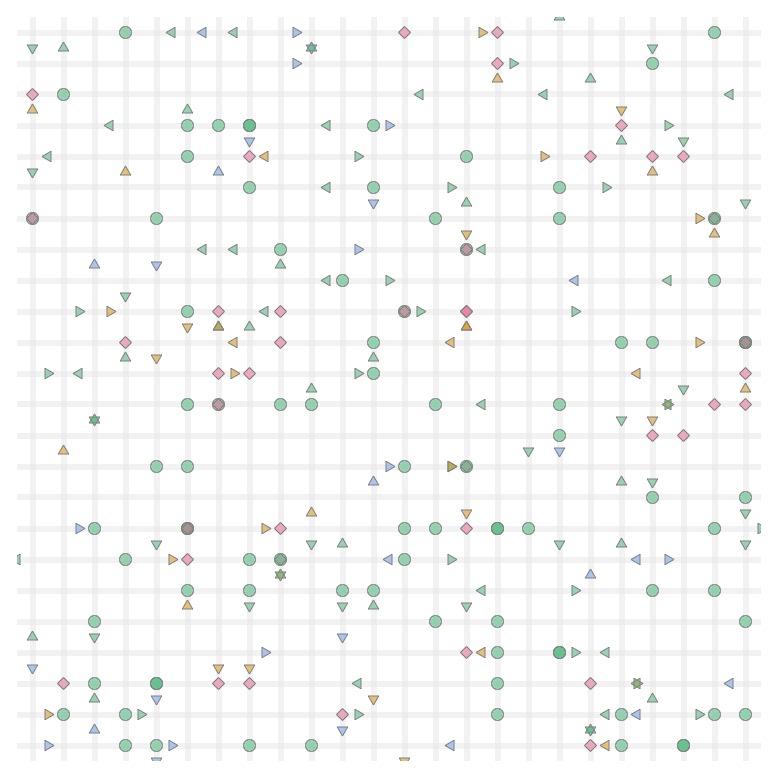
\includegraphics[width=0.7\textwidth,height=\textheight]{fig2.png}

}

\caption{\label{fig-2}A city of 20 by 20 blocks, showing 160 vehicles
(triangles) in phases \(P1\) (red), \(P2\) (orange), and \(P3\) (green).
The red diamonds are trip origins, and the green circles are trip
destinations.}

\end{figure}

At the end of each move, the simulation records and optionally plots the
state of each vehicle and statistics about the overall system (fraction
of vehicles in each phase, for example). Figure~\ref{fig-2} illustrates
a simulation in progress.

This framework is sufficient to simulate a city with a fixed supply of
vehicles, and fixed demand (rate of requests). For some of the results
below, this is all that is needed. For some other topics, the simulation
has to be extended.

\hypertarget{identities}{%
\subsection{Identities}\label{identities}}

With the trip and vehicle phases defined as they are here, there are
three identities that are always obeyed by simulations that establish a
steady state.

The first identity says that the time that vehicles spend with
passengers on board is the same as the time that passengers spend riding
in vehicles

\[
N \times P3 = D \times L
\]

where:

\begin{itemize}
\item
  \(N\) is the number of vehicles, which represents the supply of
  vehicles
\item
  \(P3\) is the fraction of time vehicles have passengers
\item
  \(D\) is the rate of trip requests, which represents the demand for
  trips
\item
  \(L\) is the average trip duration.
\end{itemize}

A second identity says that, again as long as the system is in a steady
state, the time vehicles spend \emph{en route} to trip origins is the
same as the time passengers spend waiting to be picked up.

\[
N \times P2 = D \times W
\]

where:

\begin{itemize}
\item
  \(P2\) is the fraction of time vehicles spend \emph{en route} to
  picking up passengers
\item
  \(W\) is the average wait time.
\end{itemize}

\hypertarget{extensions}{%
\subsection{Regions in the city}\label{extensions}}

The spirit of the simulation is to be as simple as possible, so that it
can be calibrated using the very limited high-level public data
available and so that it can be used comparatively. However, two
extensions are necessary for some applications.

Many cities have a central ``downtown'' zone where the demand for
ridehail traffic is high, surrounded by suburban areas where demand is
lower. For example, 60\% of trips in Metro Toronto originate within
``Old Toronto'' and East York, even though these two make up less than
20\% of the total Metro area. This inhomogeneity is built into the model
as two \emph{zones}. A central zone has sides \(C/2\) (so, one quarter
of the city's area) and has a higher rate of trip requests than the
surrounding area, as shown in Figure~\ref{fig-3} below. The trip
destinations remain randomly distributed around the whole city. With an
inhomogeneity of zero, the central zone is the same as the rest, with an
inhomogeneity of one all trip requests take place in the central zone.
In this way, and in the spirit of keeping the model as simple and
parsimonious as possible, a single inhomogeneity parameter between zero
and one captures the two zones.

\begin{figure}

{\centering 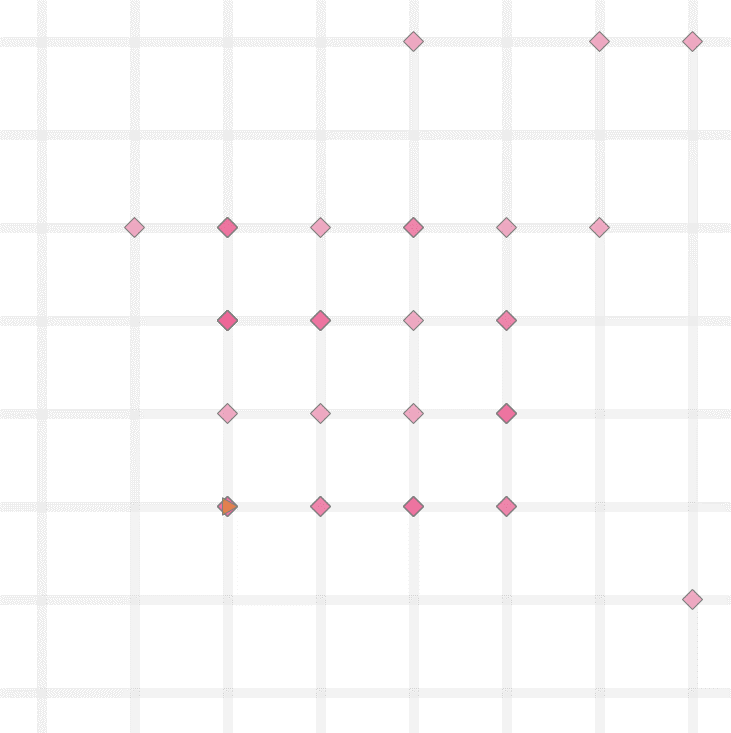
\includegraphics[width=0.5\textwidth,height=\textheight]{fig3.png}

}

\caption{\label{fig-3}The red dots show the origin of trips in a small
``two-zone'' city if eight blocks. The central area has a higher demand
than outlying suburbs.}

\end{figure}

The second extension, discussed in the section on Engaged Time standards
below, is to allow vehicles to enter and leave the system in response to
price and demand.

The use of random locations for trip destinations implies an average
trip length of \(C/2\) (regardless of inhomogeneity). To model an area
where the average trip length may differ from this, a maximum trip
length can be set, with trips distributed randomly over intersections
within that distance.

\hypertarget{equilibration}{%
\subsection{Equilibration}\label{equilibration}}

A distinguishing feature of the gig economy model is that once drivers
are signed up they are generally free to enter or leave active status
simply by opening the application. The platform's ability to expand or
shrink the supply of drivers in response to demand, whether in the short
term (``surge pricing'' and its descendants) or in the longer term
through changes in commission and incentives, has been central to their
success.

Equilibration of supply has been added to the model (vehicles entering
and leaving ``active'' status). The demand for trips is currently
treated as exogenous.

A simplified formula for average net income \(I\) is as follows:

\[
I = I_0 - c
  = P3 \cdot p \cdot (1 - f) - c
\]

where:

\begin{itemize}
\item
  \(I_0\) is gross income
\item
  \(p\) is the price of a trip (fare per block)
\item
  \(f\) is the platform commission, as a fraction of the fare
\item
  \(c\) is the marginal cost of operating the vehicle
\end{itemize}

If the average net income is above a threshold \(w_0\), called the
\emph{reservation wage}, then there is money to be made and vehicles
will enter the market. If the average net income is below the
reservation wage, some vehicles will leave. The reservation wage is
determined by external factors such as the state of the labour market,
which determines what other options are open to drivers apart from
ridehail and hence how much they have to earn in order to find ridehail
worthwhile.

If vehicles enter, the additional supply of drivers provides additional
competition for the available rides, the utilization rate \(P3\) falls,
and so the average income also falls. If vehicles leave, there is less
competition for the available rides, the utilization rate and average
income increase. When the average income matches the reservation wage,
the system is at equilibrium.

Vehicles entering and leaving the arena looks like a dynamic process,
but there is no attempt to model time in the approach to equilibrium.
The rate at which vehicles enter and leave is set purely for
convenience. In principle, the parameters could be set to describe short
term (surge pricing) or longer term equilibration (drivers deciding to
sign up to the platform or leaving it).

\hypertarget{simplification}{%
\subsection{Simplification}\label{simplification}}

The model is obviously a dramatic simplification of reality. There is no
treatment of cancelled trips, of distinctions among drivers, of
information asymmetries and special driver incentives, or of many other
factors that go to make up the complex world of ridehailing. The
distribution of trip durations is roughly normal, which is different
from the actual distribution. Most simulations are run with no account
taken for different driver speed when idle compared to when engaged on a
trip. But in some ways this oversimplification is a strength: there is
so little public data available regarding the specifics of ridehail
markets that any more complex model would be overfitted. Many published
reports and papers have relied either on access to Uber's data or on
driver surveys to collect data. The former has obvious conflict of
interest problems and the latter is always going to be partial. The
challenge, in fact, is to find enough reliable data to calibrate even
this simplified model against reality. A second benefit is that by
having a small number of parameters we can address some of the questions
asked in public and policy circles, which relate to overall gross
features of the system. How does wait time depend on demand? What are
the likely consequences of a price increase? More generally, how to the
basic variables of the system affect each other. Finally, a simple model
should allow comparison among cities, based on their values of the basic
parameters.

\hypertarget{implementation}{%
\subsection{Implementation}\label{implementation}}

The simulation is implemented in the Python programming language, and
the code is available on GitHub at
\url{https://github.com/tomslee/ridehail}. It can be run as a desktop
application from a command line (tested on Windows and on Linux) but a
subset can be explored interactively online at
\url{https://tomslee.github.io/ridehail/lab/}.

Simulations using the desktop application are controlled by a
configuration file, which at its simplest specifies the size of the city
(number of blocks on each side), the base demand rate (number of trip
requests each move), and the number of vehicles. Currently there are
almost 50 configuration parameters governing (beyond the basic
simulation), logging, animation, sequence, equilibration, shocks and
more.

A subset of the simulation is also available at a web site, where the
configuration is set in the browser. The simulation runs in the browser
(not at a server), using the Pyodide python distribution (The Pyodide
development team 2022), and is the same code as the desktop. The web
site is currently a ``laboratory'', which allows experimentation but
does not provide a way to save results. All results in this paper are
taken from desktop simulations.

\hypertarget{simulating-ridehail-in-toronto}{%
\section{Simulating ridehail in
Toronto}\label{simulating-ridehail-in-toronto}}

The ridehail market in Metropolitan Toronto was chosen as a test arena.
The city has released important data in a 2019 study by the City of
Toronto (Policy \& Innovation Transportation Services 2019) and an
update in 2021 (Policy \& Innovation Transportation Services 2021), here
called \emph{Toronto 2019} and \emph{Toronto 2021}.

Metro Toronto has a population of 3 million people. It consists of the
City of Toronto and surrounding urban areas (Scarborough, Etobicoke,
York, East York, and North York and is intermediate in size between the
old City of Toronto and the Greater Toronto Area (population 6 million).
Metro Toronto (henceforth just ``Toronto'') has an area of 630 square
kilometres ( \(\approx 25 \times 25 km\))

\hypertarget{reference-values}{%
\subsection{Reference values}\label{reference-values}}

In \emph{Toronto 2021}, the authors chose Thursday Feb 6, 2020 as a
representative day to assess the overall state of ridehail in Toronto,
pre-pandemic (p25). Can the model reproduce important aspects of this
day? Although the date is now three years in the past, any reference to
``Toronto'' here implies ``Toronto on February 6, 2020''. Relevant
statistics from this study are shown in Table 1.

\begin{longtable}[]{@{}lr@{}}
\caption{Table 1: Statistics for Uber trips in Toronto on Feb 6, 2020.
The values come from the City of Toronto study on platform transit
companies.}\tabularnewline
\toprule()
Quantity & Value \\
\midrule()
\endfirsthead
\toprule()
Quantity & Value \\
\midrule()
\endhead
Trips completed (D) & 193,902 (135/min) \\
Average trip length (L) & 8.13km \\
Average vehicle speed (v) & 31 km/h \\
Percent of time: Period 1 (available for trip) & 40.5\% \\
Percent of time: Period 2 (en-route to pick-up) & 11.2\% \\
Percent of time: Period 3 (with passenger) & 48.3\% \\
Active vehicles per hour & 6200 \\
\bottomrule()
\end{longtable}

Several adjustments are needed to turn these raw values into quantities
that can be used to calibrate the model.

There is a regular churn of active vehicles, so the reported number of
active vehicles per hour overestimates the number on the streets at any
one time. Using the distribution of vehicle hours from the Toronto 2021
report suggests that 40\% of all vehicles will leave during any given
hour, so that to maintain a steady volume of traffic a corresponding
number will enter. The number of active vehicles at any one time is
therefore 6200 * 100 / 140 = 4400.

For these numbers to fit Identity I, we take the following as reference
values:

\begin{longtable}[]{@{}
  >{\raggedright\arraybackslash}p{(\columnwidth - 4\tabcolsep) * \real{0.4795}}
  >{\centering\arraybackslash}p{(\columnwidth - 4\tabcolsep) * \real{0.2603}}
  >{\raggedleft\arraybackslash}p{(\columnwidth - 4\tabcolsep) * \real{0.2603}}@{}}
\caption{Reference values for an average hour of ridehail traffic in
Toronto on Feb 6, 2020}\tabularnewline
\toprule()
\begin{minipage}[b]{\linewidth}\raggedright
Quantity
\end{minipage} & \begin{minipage}[b]{\linewidth}\centering
Symbol
\end{minipage} & \begin{minipage}[b]{\linewidth}\raggedleft
Value
\end{minipage} \\
\midrule()
\endfirsthead
\toprule()
\begin{minipage}[b]{\linewidth}\raggedright
Quantity
\end{minipage} & \begin{minipage}[b]{\linewidth}\centering
Symbol
\end{minipage} & \begin{minipage}[b]{\linewidth}\raggedleft
Value
\end{minipage} \\
\midrule()
\endhead
Average number of active vehicles & \(N\) & 4500 \\
Demand (trip requests per minute) & \(D\) & 135 per minute \\
Average trip duration & \(L\) & 16 minutes \\
Percent of time: Period 1 (available for trip) & \(P1\) & 40.5\% \\
Percent of Percent of time: Period 2 (en-route to pick-up) & \(P2\) &
11.2\% \\
Percent of time: Period 3 (with passenger) & \(P3\) & 48.3\% \\
Average wait time & \(W\) & 3.7 minutes \\
Average wait fraction & \(W / L\) & 0.23 \\
\bottomrule()
\end{longtable}

\hypertarget{calibration-i-supply-demand-and-utilization-rate}{%
\subsection{Calibration I: supply, demand, and utilization
rate}\label{calibration-i-supply-demand-and-utilization-rate}}

At 31 km/hour, it takes 48.4 minutes to cross the city. In the
simulation Toronto is represented as a 48 by 48 grid, so that each block
represents a minute of travel. Trips start and finish at random
locations but with a maximum duration of 32 minutes, which yields an
average duration of 16 minutes to match the observed duration. The
demand for trips was fixed at the observed average value of 135 trips
per minute.

\begin{figure}

{\centering 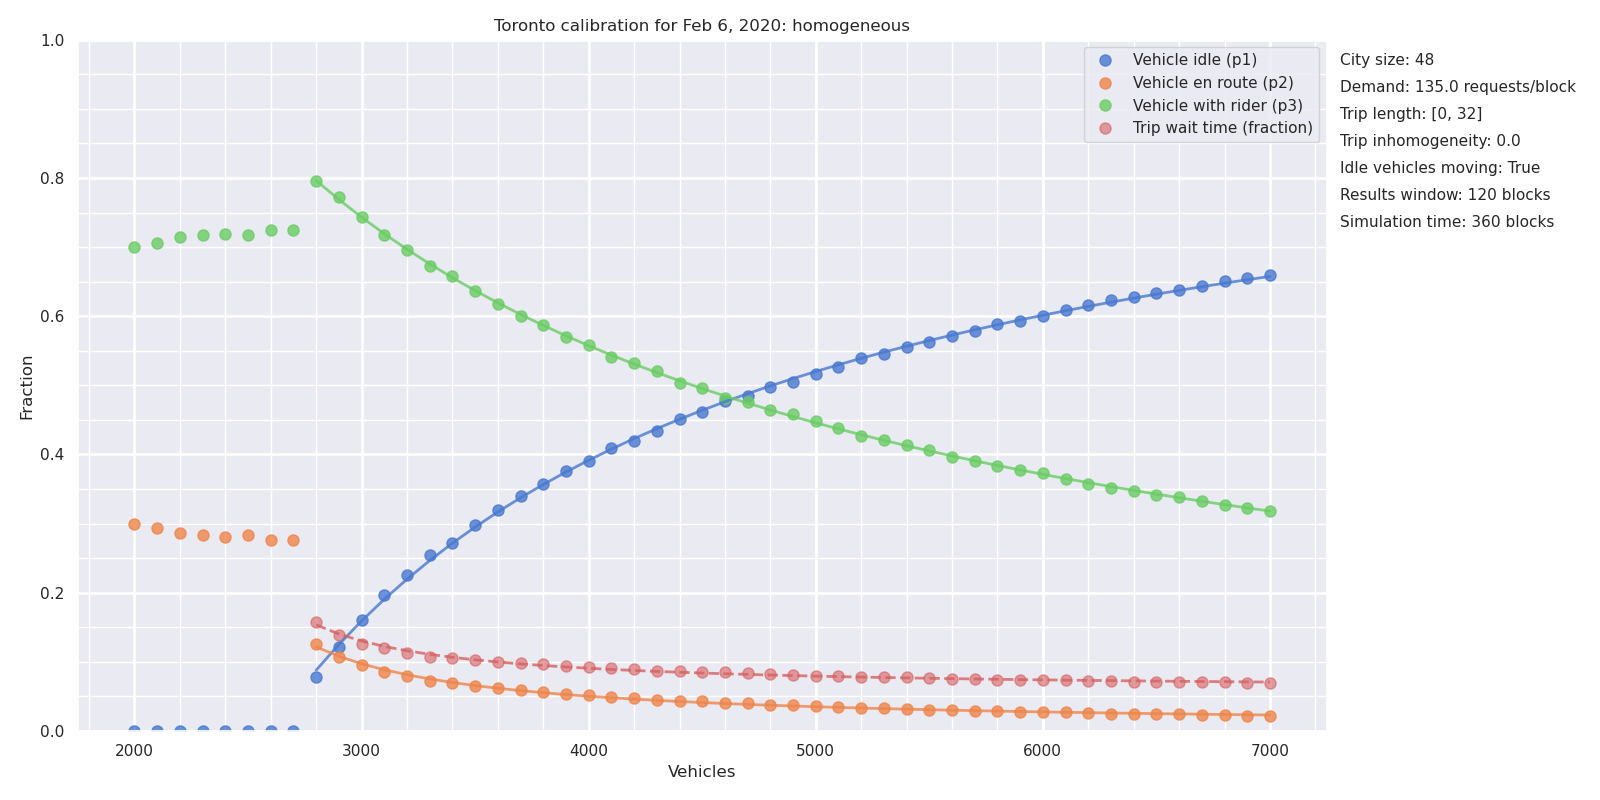
\includegraphics{toronto_calibration_homogeneous.png}

}

\caption{\label{fig-toronto-homogeneous}First calibration of Toronto
ridehail simulation: homogeneous model}

\end{figure}

Figure~\ref{fig-toronto-homogeneous} shows the results of a sequence of
simulations, with the number of vehicles varied from 2000 to 7,000. For
each value of \(N\), a simulation of 500 blocks duration was carried
out, with the results averaged over the final 100 blocks. The time for
each simulation depends on the number of vehicles: for 5000 vehicles the
simulation takes about NN minutes on a Dell XPS 13 9380 laptop: this
simplified model can simulate an environment the scale of Toronto on a
single laptop computer.

At low vehicle counts, there are too few vehicles to sustain a steady
state. Vehicles are busy all the time (\(P1 = 0\)), trip requests go
unanswered for longer and longer (the wait fraction \(W\) is literally
off the chart. Things fall apart: the drivers cannot keep up with the
requests.

At vehicle counts above 3000, a steady state is achieved. With more
vehicles, the utilization rate \(P3\) falls and the excess capacity
\(P1\) rises, as more vehicles compete for the available trips. The wait
time \(W\) does decrease as the number of vehicles increases, but is a
small fraction of the trip duration even at 3000 vehicles, and the
dispatch time \(P2\) is correspondingly low.

This model correctly reproduces the \(P3\) value of 0.48 with a supply
of \(N = 4500\) vehicles. In some ways this is just a check that
eliminates some bugs: the identity is satisfied by any steady-state
behavior, regardless of geometry. The chart confirms that the
utilization rate depends solely on vehicle supply \(N\), trip demand
\(D\), and trip duration \(L\), but not on finer features of the city
geography.

\hypertarget{calibration-ii-wait-times-and-dispatch-times}{%
\subsection{Calibration II: wait times and dispatch
times}\label{calibration-ii-wait-times-and-dispatch-times}}

The homogeneous model of Toronto, with trip origins and destinations
distributed randomly over the whole city, delivers the correct ratio of
\(P3\) to \(N\). However, the homogeneous model underestimates dispatch
time \(P2\) and wait time \(W\) compared to the observed results.
Identity II fixes the \(W/P2\) ratio, but not the absolute value of
either of those quantities. To get this value correct we must allow
inhomogeneity of trip distributions.

\begin{figure}

{\centering 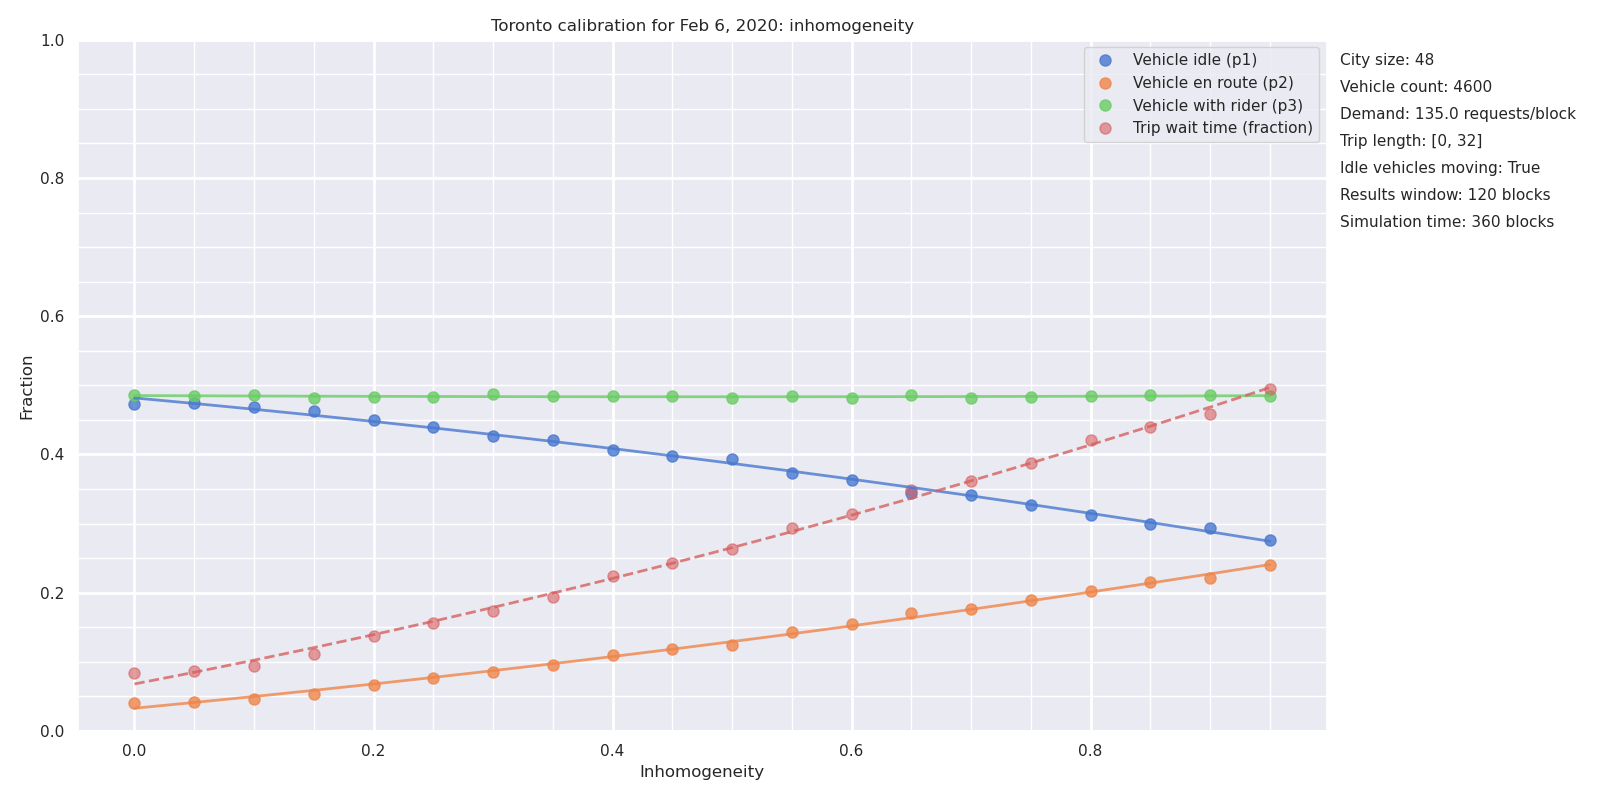
\includegraphics{toronto_calibration_inhomogeneous.png}

}

\caption{\label{fig-inhomog}Second step of Toronto ridehail calibration:
wait times and inhomogeneity}

\end{figure}

Figure~\ref{fig-inhomog} shows the vehicle phases as a function of
inhomogeneity, using the fixed demand of 135 trips per minute and a
fixed supply of 4500 vehicles derived from
Figure~\ref{fig-toronto-homogeneous}. The Figure shows that the
utilization rate \(P3\) is independent of inhomogeneity, as expected. An
inhomogeneity of 0.4 reproduces the observed values of \(P2\) and \(W\),
and hence \(P1\), completing the essential descriptive statistics of
Toronto's ridehail market.

An inhomogeneity of 0.4 means that 60\% of trip origins are distributed
randomly over the entire city, while 40\% are constrained to within the
central square, of size \(C/2 \times C/2\). Hence, 55\% of all trips
start in the central ``downtown area''. This corresponds roughly to the
old City of Toronto (reference needed for travel times).

\hypertarget{the-tension-between-wait-times-and-excess-capacity}{%
\subsection{The tension between wait times and excess
capacity}\label{the-tension-between-wait-times-and-excess-capacity}}

Figure~\ref{fig-toronto-final} shows simulations for the calibrated
Metro Toronto model, with varying numbers of vehicles \(N\) from 2000 to
7000. The actual number on Feb 6, 2020 was \(N=4500\), as discussed
above.

\begin{figure}

{\centering 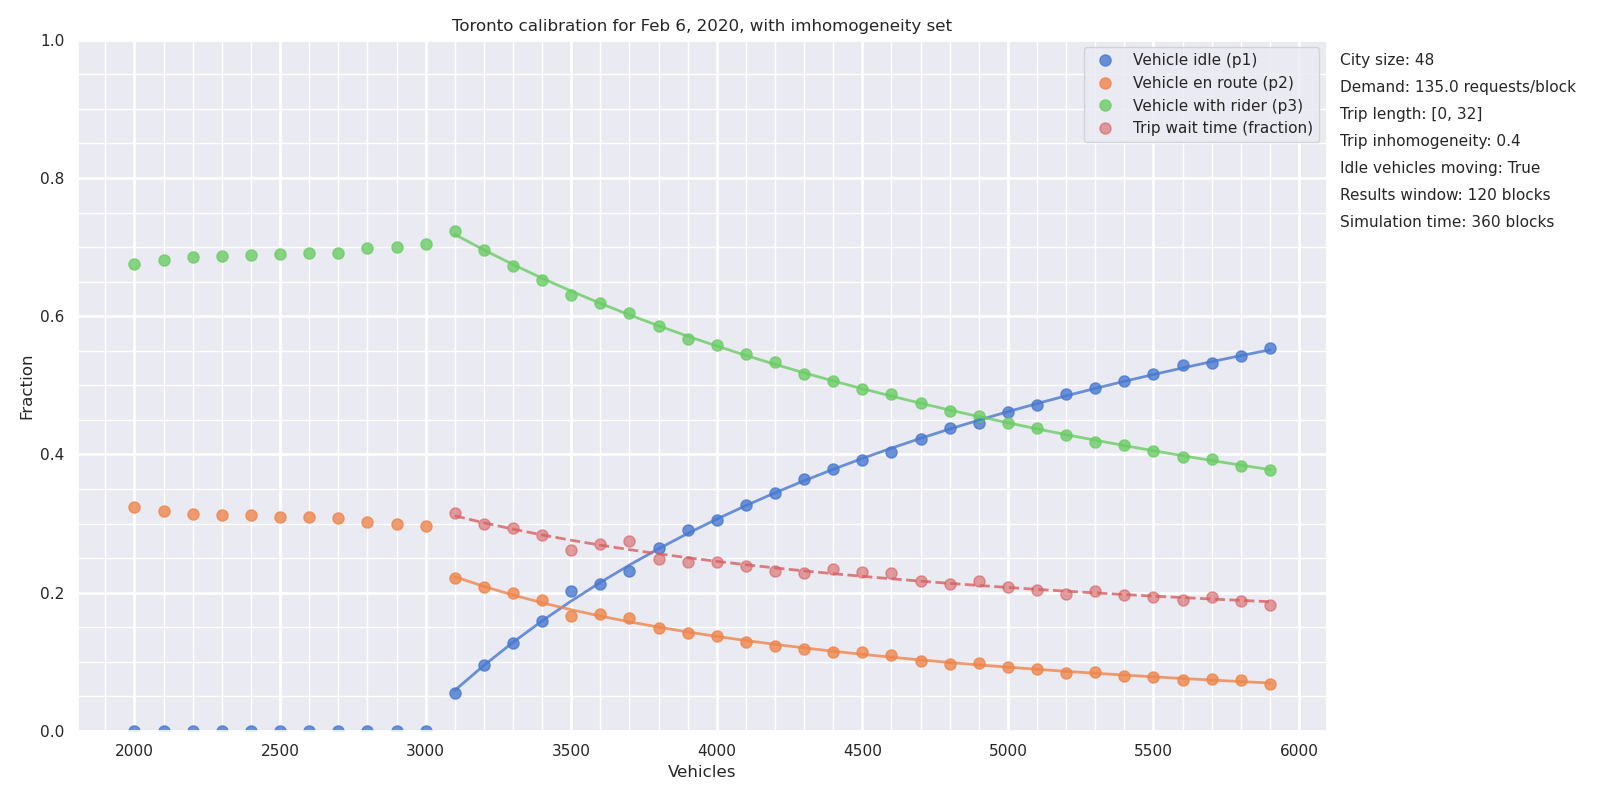
\includegraphics{toronto_vehicle_count.png}

}

\caption{\label{fig-toronto-final}How things depend on vehicle count}

\end{figure}

The model makes explicit and quantitative the trade-off between short
wait times and additional vehicles on the streets.
Figure~\ref{fig-toronto-final} shows that a decrease in wait times of
one minute (from 4.2 to 3.2 minutes, or \(W\) = 0.26 to 0.20, bracketing
the observed average of 3.7 minutes), at a fixed demand of 135 trips per
minute, adds approximately 1500 vehicles to the streets (from 3800 to
5300) with attendant congestion and pollution.

\hypertarget{does-increased-volume-produce-higher-utilization-rates}{%
\subsection{Does increased volume produce higher utilization
rates}\label{does-increased-volume-produce-higher-utilization-rates}}

In 2017, the New York Times published a story that highlighted the
tradeoff between wait times and utilization rates, including an
animation that inspired the model presented here. Uber responded with a
blog post claiming that the story missed the effect of demand: that with
additional demand, both wait times and utilization rates could increase
in a virtuous cycle. While Uber provided charts to back up the claim,
they noticeably lacked any numbers on the Y axes. Since that time, there
has been little discussion of the claim.

Figure~\ref{fig-fixed-wait-time} shows the utilization rates and vehicle
counts required to sustain a 3.7 minute wait time \$W\$ in Toronto.

\begin{figure}

{\centering 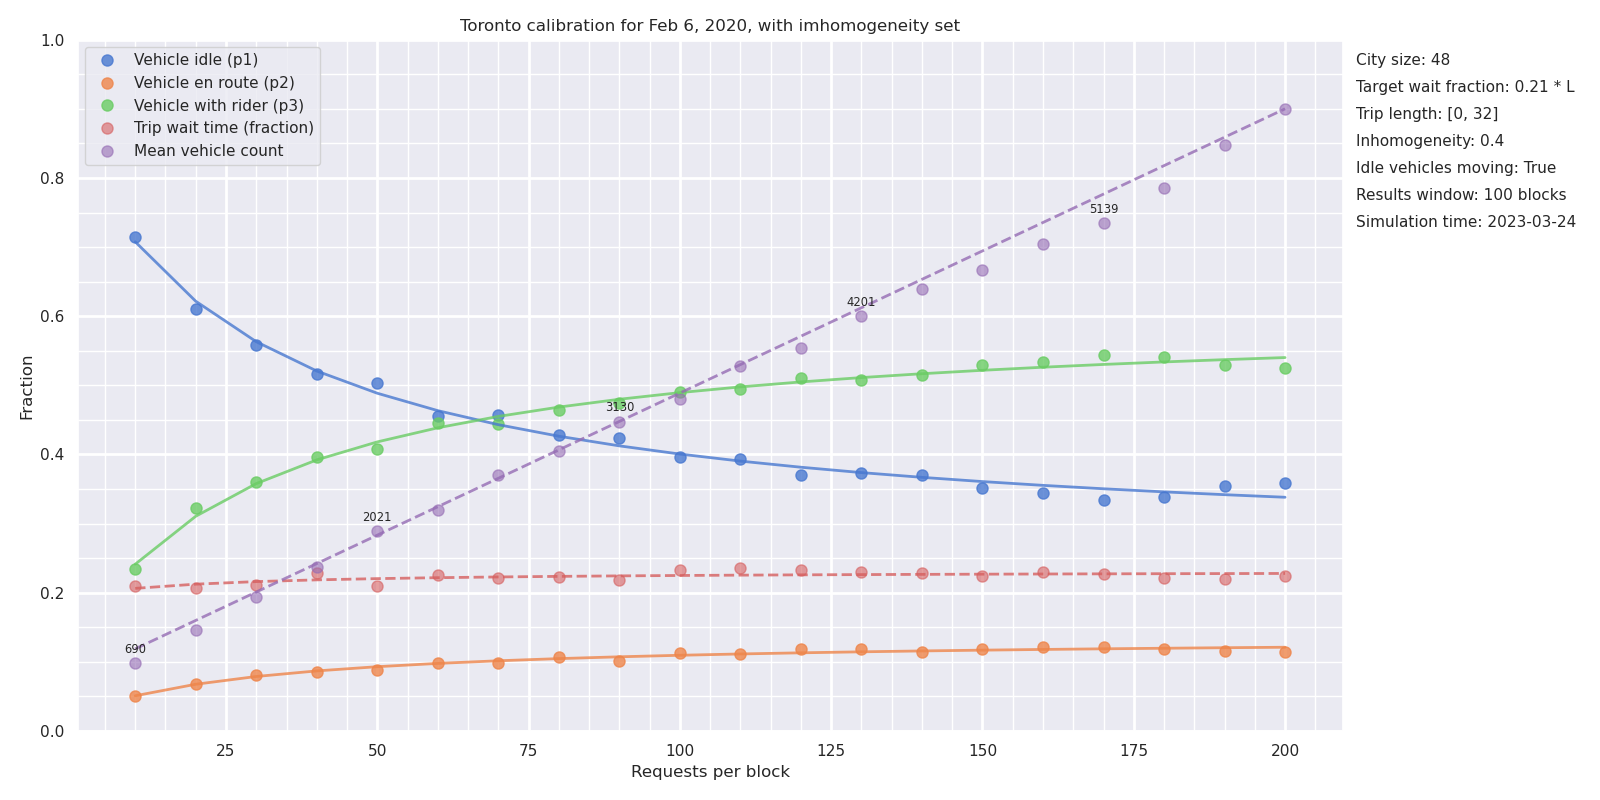
\includegraphics[width=1\textwidth,height=\textheight]{wait_times.png}

}

\caption{\label{fig-fixed-wait-time}The number of vehicles \(N\) and
utilization rate \(P3\) required to support a wait time of 3.7 minutes
(\(W =0.23\)). While the utilization rate (\(P3\)) does increase with
demand, the improvements level off at levels of demand far below the
current Toronto level of 135 requests per minute. Meanwhile, the number
of vehicles required keeps growing linearly (purple line: different
axis).}

\end{figure}

\begin{longtable}[]{@{}lllr@{}}
\caption{Table 2: Utilization rates for Uber in USA cities. Rates
measured by distance will be higher than those measured by time as
drivers cover more distance in a given time when engaged in a trip. 2019
values are from an Uber-commissioned report (Balding et al. 2019); 2017
values from a report by Bruce Schaller (Schaller 2017), and 2015 values
from an NBER report by (Cramer and Krueger 2016). The 2020 values for
Seattle come from reports by (Hyman et al. 2020) and by (Parrott and
Reich 2020).}\tabularnewline
\toprule()
City & Year & Time or distance? & Utilization rate \\
\midrule()
\endfirsthead
\toprule()
City & Year & Time or distance? & Utilization rate \\
\midrule()
\endhead
Chicago & 2015 & Distance & 59\% \\
Chicago & 2019 & Distance & 55\% \\
Boston & 2016 & Time & 47\% \\
Boston & 2019 & Distance & 55\% \\
Los Angeles & 2016 & Time & 42\% \\
Los Angeles & 2019 & Distance & 60\% \\
New York City & 2016 & Time & 51\% \\
New York City & 2017 & Distance & 59\% \\
San Francisco & 2016 & Time & 55\% \\
San Francisco & 2017 & Distance & 67\% \\
San Francisco & 2019 & Distance & 64\% \\
Seattle & 2016 & Time & 44\% \\
Seattle & 2019 & Distance & 53\% \\
Seattle & 2020a & Time & 60\% \\
Seattle & 2020b & Time & 51\% \\
Washington DC & 2019 & Distance & 55\% \\
\bottomrule()
\end{longtable}

Figure~\ref{fig-fixed-wait-time} shows that an increase in demand does
increase utilization, but that utilization levels off as demand
increases. Even if the trip volume in Toronto were to increase to
200,000 per day (a 50\% increase over the pre-pandemic numbers), the
utilization rate would still increase to only 54\% if wait time were
kept at the same value. Other cities, with New York City and San
Francisco as outliers, have utilization rates (by time) of 50 to 60\%.
Toronto has a level of demand that is lower than Chicago, which may
provide a reasonable upper bound to what can be expected of around 60\%.

There are two ways that utilization rates may exceed these estimates.
The first is for the number of drivers to be limited, so that wait times
are longer. The second is for trips to concentrate even more heavily
into the high traffic central zone. But this central core is well served
by mass transit, and any gain in ridehail trips would be achieved by
taking riders away from mass transit and putting them in cars (Young,
Allen, and Farber 2020), and adding to problems of congestion (Erhardt
et al. 2019).

Without these changes, the ridehail system has at least 40\% excess
capacity (vehicles not engaged in driving passengers or en route to pick
passengers). There is no efficient solution to emissions through ride
hailing.

\hypertarget{references}{%
\section*{References}\label{references}}
\addcontentsline{toc}{section}{References}

\hypertarget{refs}{}
\begin{CSLReferences}{1}{0}
\leavevmode\vadjust pre{\hypertarget{ref-balding2019}{}}%
Balding, Melissa, Teresa Whinery, Eleanor Leshner, and Eric Womeldohrf.
2019. {``Estimated TNC Share of VMT in Six US Metropolitan Regions.''}
\url{https://drive.google.com/file/d/1FIUskVkj9lsAnWJQ6kLhAhNoVLjfFdx3/view?usp=embed_facebook}.

\leavevmode\vadjust pre{\hypertarget{ref-cityofchicago2022}{}}%
City of Chicago. 2022. {``Transportation Network Providers - Trips.''}
\url{https://data.cityofchicago.org/Transportation/Transportation-Network-Providers-Trips/m6dm-c72p}.

\leavevmode\vadjust pre{\hypertarget{ref-cramer2016}{}}%
Cramer, Judd, and Alan B Krueger. 2016. {``Disruptive Change in the Taxi
Business: The Case of Uber.''}

\leavevmode\vadjust pre{\hypertarget{ref-erhardt2019}{}}%
Erhardt, Gregory D., Sneha Roy, Drew Cooper, Bhargava Sana, Mei Chen,
and Joe Castiglione. 2019. {``Do Transportation Network Companies
Decrease or Increase Congestion?''} \emph{Science Advances} 5 (5):
eaau2670. \url{https://doi.org/10.1126/sciadv.aau2670}.

\leavevmode\vadjust pre{\hypertarget{ref-hyman2020}{}}%
Hyman, Louis, Erica L. Groshen, Adam Seth Litwin, Martin T. Wells,
Kwelina P. Thompson, and Kyrylo Chernyshov. 2020. {``Platform Driving In
Seattle,''} July. \url{https://ecommons.cornell.edu/handle/1813/74305}.

\leavevmode\vadjust pre{\hypertarget{ref-newyorkcityopendata2022}{}}%
New York City Open Data. 2022. {``Uber Data.''}
\url{https://data.cityofnewyork.us/Transportation/uber-Data/gre9-vvjv}.

\leavevmode\vadjust pre{\hypertarget{ref-parrott2020}{}}%
Parrott, James A., and Michael Reich. 2020. {``A Minimum Compensation
Standard for Seattle TNC Drivers.''}
\url{https://irle.berkeley.edu/files/2020/07/Parrott-Reich-Seattle-Report_July-2020.pdf}.

\leavevmode\vadjust pre{\hypertarget{ref-policyinnovationtransportationservices2019}{}}%
Policy \& Innovation Transportation Services. 2019. {``The
Transportation Impacts of Vehicle-for-Hire in the City of Toronto.''}
\url{https://www.toronto.ca/wp-content/uploads/2019/06/96c7-Report_v1.0_2019-06-21.pdf}.

\leavevmode\vadjust pre{\hypertarget{ref-policyinnovationtransportationservices2021}{}}%
---------. 2021. {``The Transportation Impacts of Vehicle-for-Hire in
the City of Toronto: October 2018 to July 2021.''}
\url{https://www.toronto.ca/wp-content/uploads/2021/11/98cd-VFHTransportationImpacts2021-11-23.pdf}.

\leavevmode\vadjust pre{\hypertarget{ref-schaller2017}{}}%
Schaller, Bruce. 2017. {``Unsustainable? The Growth of App-Based Ride
Services and Traffic, Travel and the Future of New York City.''}
\url{http://www.schallerconsult.com/rideservices/unsustainable.pdf}.

\leavevmode\vadjust pre{\hypertarget{ref-thepyodidedevelopmentteam2022}{}}%
The Pyodide development team. 2022. \emph{Pyodide/Pyodide}. Zenodo.
\url{https://doi.org/10.5281/zenodo.5156931}.

\leavevmode\vadjust pre{\hypertarget{ref-young2020}{}}%
Young, Mischa, Jeff Allen, and Steven Farber. 2020. {``Measuring When
Uber Behaves as a Substitute or Supplement to Transit: An Examination of
Travel-Time Differences in Toronto.''} \emph{Journal of Transport
Geography} 82 (January): 102629.
\url{https://doi.org/10.1016/j.jtrangeo.2019.102629}.

\end{CSLReferences}



\end{document}
